Usando el principio de Cavalieri, calcula el volumen de la estructura mostrada
en la figura; cada sección de cruce es un rectángulo de longitud 5 y ancho 3.
\begin{figure}[H]
    \begin{center}
        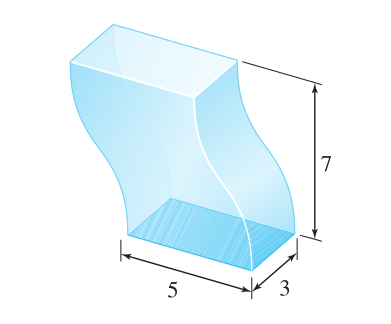
\includegraphics[width=0.3\textwidth]{img/Ej2/ej6.png}
    \end{center}
\end{figure}
\begin{solution}
    Sea $A(h)$, el área de la sección de cruce rectangular en la altura $h$. El principio 
    de Cavalieri dice que 
    el volumen de esta estructura es
    \begin{align*}
        \int_{0}^7 A(h) \, dh
        &=
        \int_{0}^7 5\cdot 3 \, dh\\
        &=
        15 \int_0^7 \, dh\\
        &=
        15 (7-0)=105.
    \end{align*}
\end{solution}
